En esta sección se muestran las distintas pruebas de validación que se han realizado a la aplicación. Por una parte se ha realizado una evaluación del modelo NLU para comprobar como se comporta el modelo, y por otra, un estudio de usabilidad con \textit{feedback} de usuarios reales.\\
 

\section{Evaluación del modelo NLU}
Una vez el chatbot está publicado, este recibe y procesa información que no forma parte de su conjunto de entrenamiento. Para observar como se comportará el modelo bajo estas circunstancias es posible evaluar el modelo de comprensión del lenguaje natural (NLU). Para ello, previamente se divide el \textit{dataset} en una proporción de 80/20 de datos de entrenamiento y de test respectivamente. Tras esta división, se realiza un entrenamiento con los datos destinados al entrenamiento y se prueba el modelo con los datos de test. En esta prueba, \textit{Rasa} comprobará si el modelo identifica correctamente los \textit{intents}.\\     

\begin{figure}[htbp]
\centering
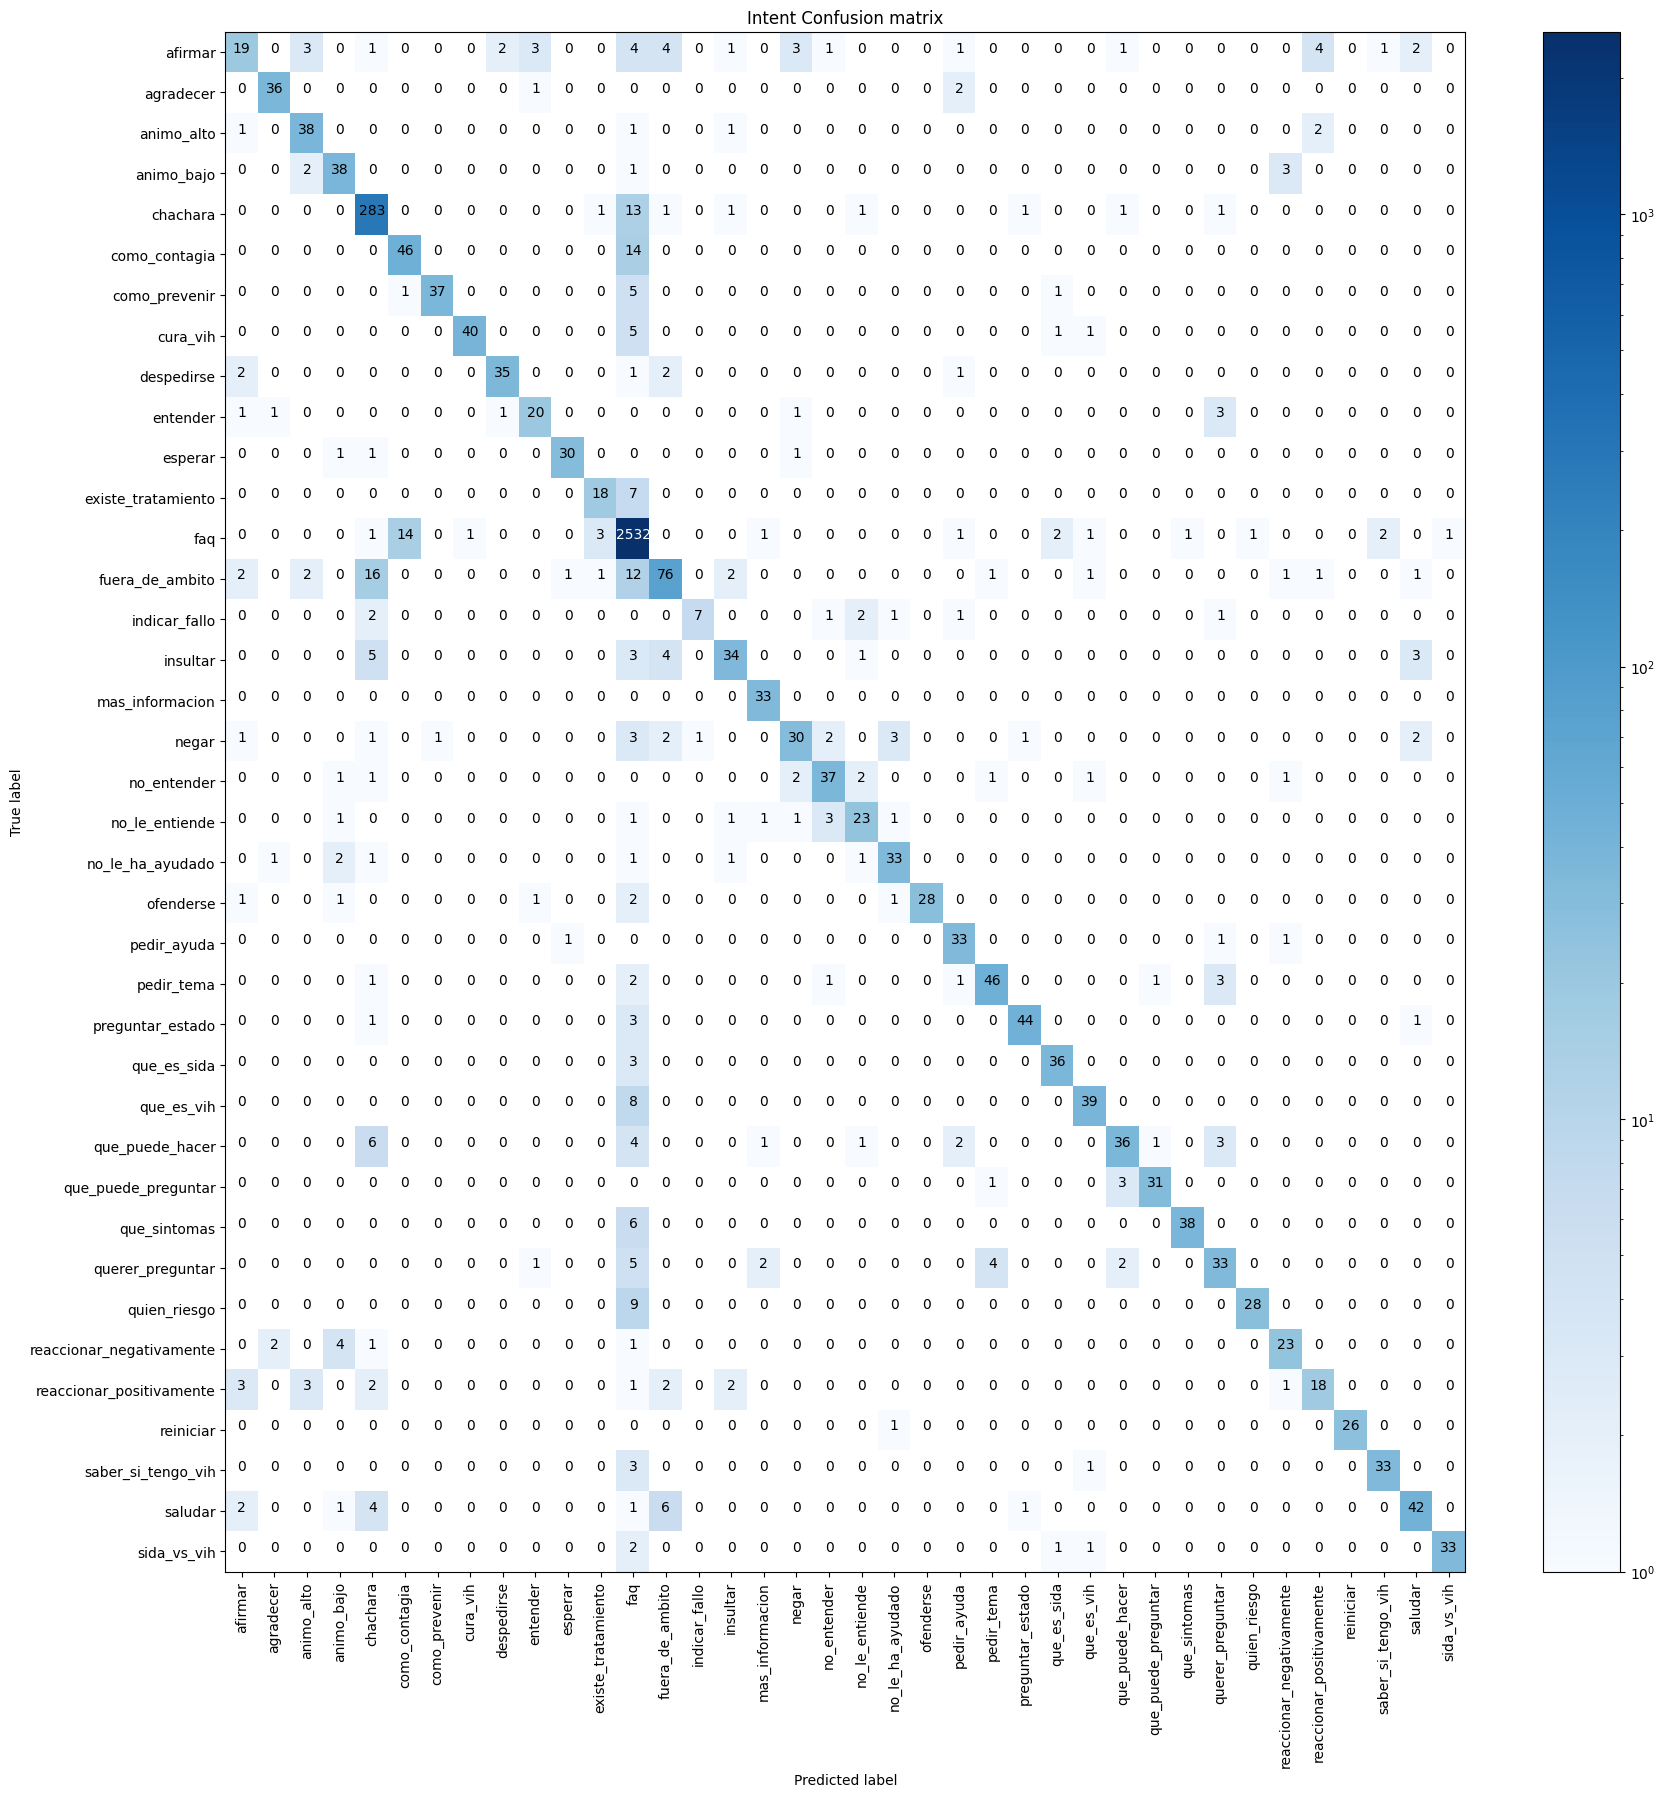
\includegraphics[scale=0.4]{../images/intent_confusion_matrix.png}
\caption{Matriz de confusión de \textit{intents}}
\label{fig:intentconfusion}
\end{figure}
Tras realizar el test, se obtiene un informe con los resultados. El informe consta de un archivo en formato \textit{JSON} y una matriz de confusión de \textit{intents}. En la Figura \ref{fig:intentconfusion} se puede observar la matriz de confusión obtenida tras el test. Idealmente, si no se produjera ninguna confusión entre \textit{intents}, debería ser una matriz diagonal. En este caso, aunque gran parte de los datos se concentran en la diagonal (indicando la correcta identificación de un \textit{intent}), si que podemos observar algo de dispersión. Por ejemplo, es significativa la confusión que se produce entre el \textit{intent} \textit{chachara} y \textit{fuera de ámbito}. Esta confusión se puede deber a la similitud de los datos entre ambos intents, ya que tanto la conversación informal como las expresiones fuera del ámbito del chatbot pueden tener características similares.\\

 %y un histograma de la distribución de la confianza con la cual se han identificado los \textit{intents}.\\
 


Por otra parte, también podemos observar como muchos datos son identificados erróneamente como \textit{faq}. El término \textit{faq} es el \textit{intent} donde se agrupan la mayor parte de \textit{subintents} relacionados con el VIH. Por tanto, es donde más variedad de datos se concentra, dando lugar a las confusiones que muestra la matriz. Por tanto, la evaluación del modelo NLU ha servido para revisar el rendimiento del modelo e identificar que \textit{intents} han dado problemas de confusión. Tras su detección, se ha procedido a la revisión de la calidad de los datos del conjunto de entrenamiento y se han realizado las modificaciones oportunas.\\

%\begin{figure}[htbp]
%\centering
%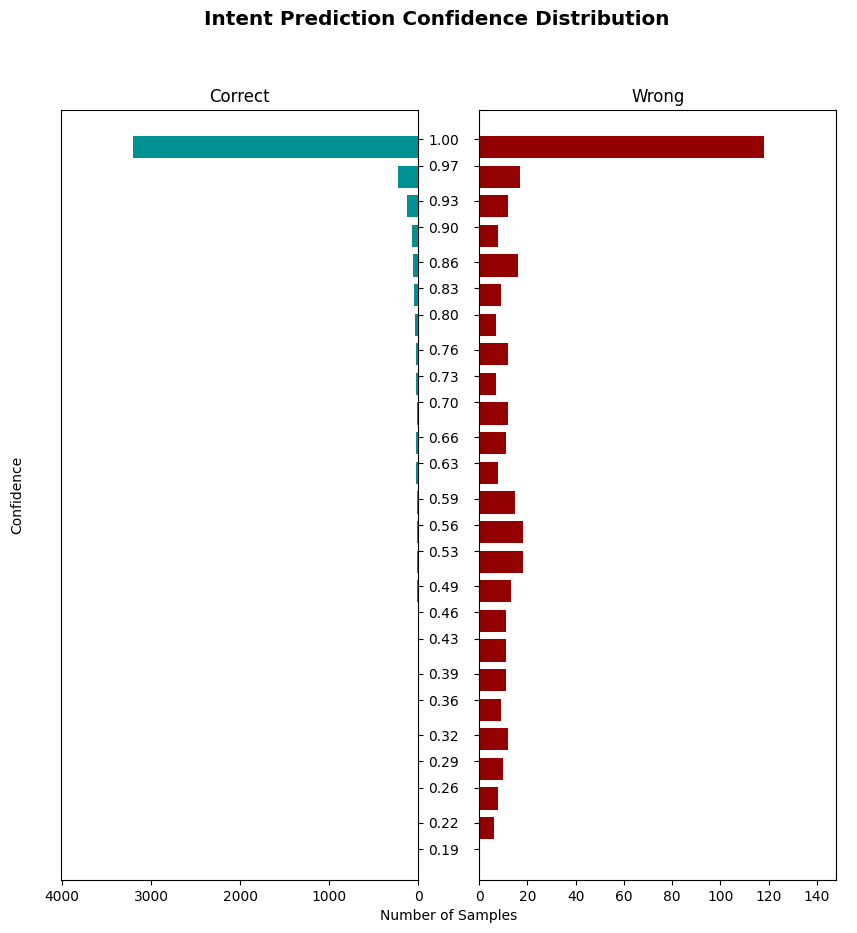
\includegraphics[scale=0.4]{../images/intent_histogram.png}
%\caption{Histograma de la distribución de confianza}
%\label{fig:histogram}
%\end{figure}

\section{Evaluación de usabilidad}
Con la finalidad de validar el correcto funcionamiento del asistente virtual, se ha realizado una prueba de usabilidad con usuarios reales. De esta manera, se podrían detectar posibles errores y corregirlos. Los participantes fueron mayoritariamente estudiantes de la UPV, captados a través de una invitación por email enviada por los tutores de este trabajo. El correo incluía un breve texto indicando a los participantes que probaran durante unos minutos el chatbot y que, posteriormente, realizaran un cuestionario facilitado a través de un link. Todos los participantes que realizaron el cuestionario han sido incluidos en los resultados. En total, 12 adultos participaron en la prueba durante un periodo de 7 días.\\

Para este estudio se han utilizado los cuestionarios validados \textit{System Usability Scale} (SUS) \cite{dirtySUS} y \textit{Chatbot Usability Questionnaire} (CUQ) \cite{cuq}. SUS es un cuestionario genérico diseñado para obtener una evaluación general y rápida sobre la usabildiad de una determinada aplicación \cite{dirtySUS}. Se compone de 10 afirmaciones sobre las cuales los usuarios deben valorar en una escala del 1 al 5 su total disconformidad (1) o total conformidad (5). Se utilizó una versión del SUS traducida al español y validada \cite{spanishSUS}.\\

Por otro lado, CUQ es un cuestionario de usabilidad específico que evalúa la personalidad, la inteligencia, el entendimiento, la navegación y el manejo de errores de un chatbot \cite{cuq}. CUQ está diseñado para ser comparable al SUS (utiliza la misma escala de valoración) pero utilizando 16 afirmaciones específicas para chatbots. Para su uso, se realizó una traducción lo más fiel posible al español.\\

Ambos cuestionarios fueron realizados a través de herramienta \textit{Google Forms} y en los anexos a este documento se puede encontrar un documento con las preguntas y respuestas obtenidas.

\subsection{Cálculo de puntuaciones}
Una vez recogidos todos los datos, se utilizó la hoja de cálculo de puntuación SUS \cite{susSpread} para calcular las puntuaciones sobre 100. La fórmula para este cálculo se muestra en la ecuación \ref{eqSus}.\\

\begin{equation}
\overline{SUS} = \frac{1}{n} \sum_{i=1}^{n}norm. \sum_{j=1}^{m} \left\{
    \begin{array}{ll}
        q_{i,j}-1,q_{i,j} mod2>0 \\
        5-q_{i,j,otherwise.}
    \end{array}
\right.
\label{eqSus}
\end{equation}

donde n=número de sujetos (cuestionarios), m=10 (número de preguntas), q\textsubscript{i,j}=puntuación individual por pregunta por participante y norm=2.5.\\

Las puntuaciones del CUQ se calcularon sobre 160 utilizando la hoja de cálculo de puntuación CUQ \cite{cuqCalc}. Posteriormente, los resultados se normalizaron para dar una puntuación sobre 100, permitiendo así la comparación con SUS. La fórmula para el cálculo se muestra en la ecuación \ref{eqCuq}.\\


\begin{equation}
CUQ = \frac{(\sum_{i=1}^{m}2p_{i}-1)-8)+40-(\sum_{n=i}^{m}2p_{i})}{64} \times 100
\label{eqCuq}
\end{equation}
% CUQ ((((P1+P3+P5+P7+P9+P11+P13+P15)-8)+(40-(P2+P4+P6+P8+P10+P12+P14+P16)))/64)*100


donde m = 16 (número de preguntas) y p\textsubscript{i} = puntuación de cada pregunta individual por participante \cite{cuq}.\\

\subsection{Resultados}

A continuación se exponen los resultados obtenidos de los 12 participantes que evaluaron la usabilidad de Vihrtual-App.\\

\subsubsection{\textit{System Usability Scale (SUS)}}
En la Figura \ref{fig:susplot} se muestra un diagrama de \textit{box and whisker} con las puntuaciones que recibió la aplicación en el cuestionario SUS. La puntuación media fue de 85.625 sobre 100. La puntuación máxima obtenida fue de 97.5 y la mínima de 65.0. La puntuación media de VIHrtual-App sitúa al chatbot en el rango del percentil 96 al 100, equivalente al \textit{Grado A+} \cite{susResults}. Si se observan los resultados desglosados por prueba y participante (ver documentos anexos a este trabajo), se puede comprobar como, al igual que en la valoración global, todos los participantes arrojaron una puntuación en SUS superior a la CUQ. Esto puede deberse a que SUS pueda ser menos efectivo para evaluar la usabilidad de un chatbot, pues sus preguntas son más genéricas y están orientadas a medir aspectos más tradicionales del \textit{UX}.\\

\begin{figure}[htbp]
\centering
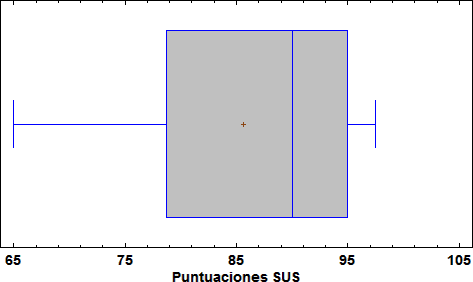
\includegraphics[scale=0.8]{../images/sus.png}
\caption{Puntuaciones SUS de Vihrtual-App}
\label{fig:susplot}
\end{figure}

\subsubsection{\textit{Chatbot Usability Questionnaire (CUQ)}}
En la Figura \ref{fig:cuqplot} se muestra un diagrama de \textit{box and whisker} con las puntuaciones que recibió el chatbot en el cuestionario CUQ. La puntuación media fue de 80.342. La puntuación máxima obtenida fue de 95.3 y la mínima de 65.6. Tal y como se ha mencionado anteriormente, la puntuación media de CUQ es inferior a la SUS, y por tanto, sitúa al chatbot en el rango del percentil 90 al 95, equivalente al \textit{Grado A}.

\begin{figure}[htbp]
\centering
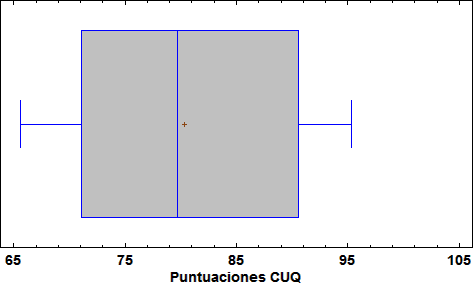
\includegraphics[scale=0.8]{../images/cuq.png}
\caption{Puntuaciones CUQ de Vihrtual-App}
\label{fig:cuqplot}
\end{figure}


Por su parte, CUQ está orientado específicamente a chatbots y permite obtener detalles muy relevantes sobre ciertos aspectos de VIHrtual-App. En este sentido, ha sido notable la valoración positiva sobre la personalidad del chatbot. Como se puede observar en la Figura \ref{fig:encuesta}, en una escala del 1 (Totalmente en desacuerdo) al 5 (Totalmente de acuerdo) un 83.4\% (66.7\% + 16.7\%) de los participantes expresó estar muy conforme con la afirmación \textit{La personalidad del chatbot era real y cautivadora}.\\

\begin{figure}[htbp]
\centering
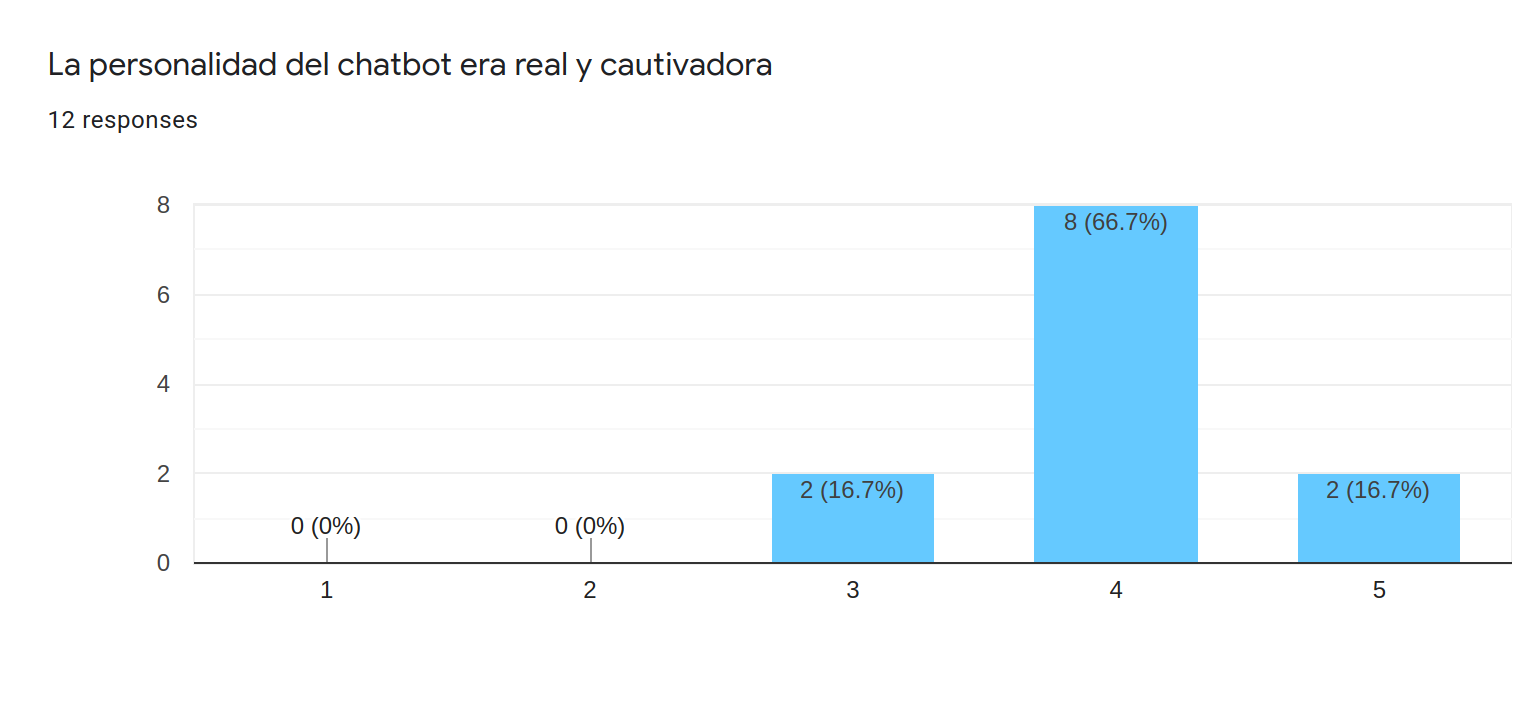
\includegraphics[scale=0.3]{../images/pregunta1.png}
\caption{Valoración de respuesta}
\label{fig:encuesta}
\end{figure}


Por otra parte, el estudio también ha revelado varios aspectos donde se necesita mejorar la experiencia de usuario. Por ejemplo, es significativo observar en la Figura \ref{fig:encuesta2} las distntas valoraciones obtenidas sobre las afirmaciones \textit{El chatbot falló en reconocer muchas de mis entradas} y \textit{El chatbot me entendió bien}.\\
 
 
\begin{figure}[htbp]
\centering
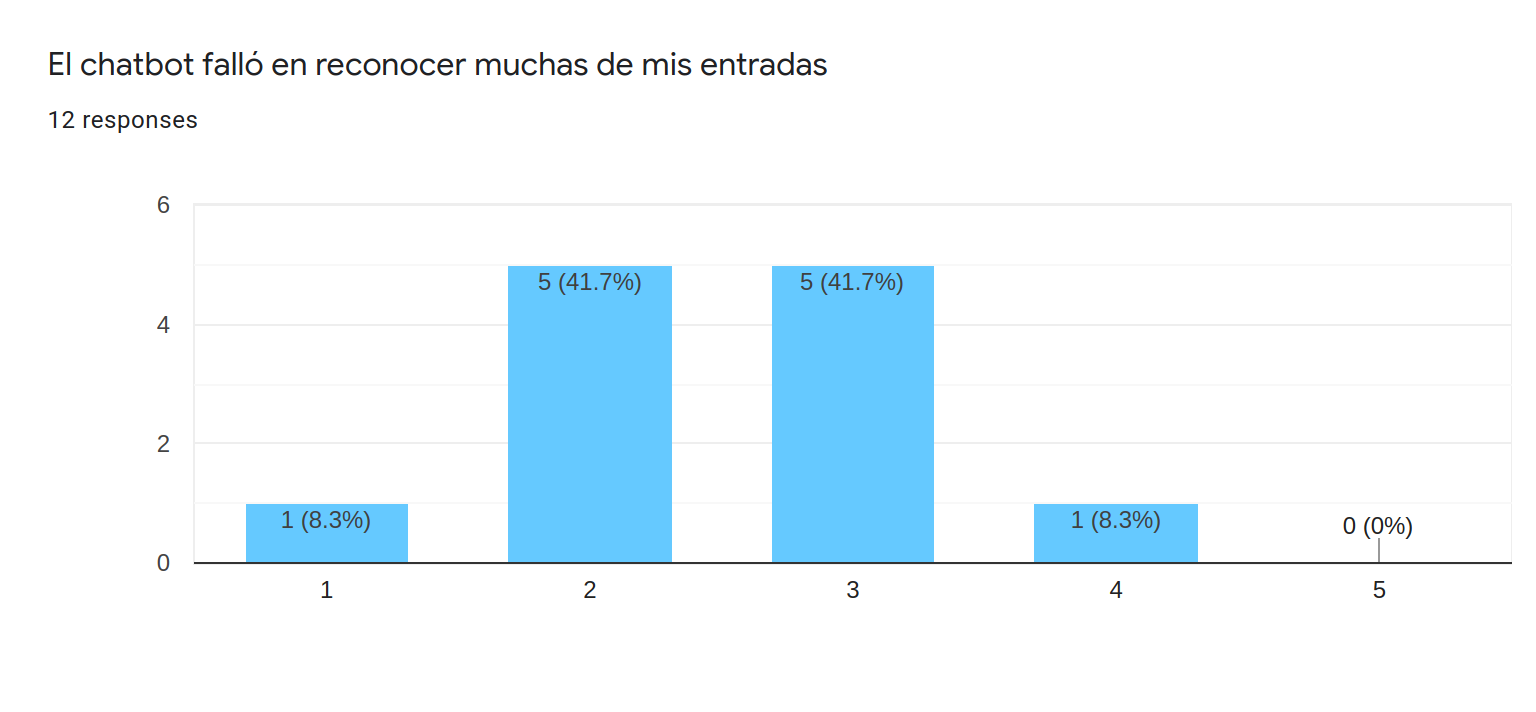
\includegraphics[scale=0.3]{../images/pregunta2.png}
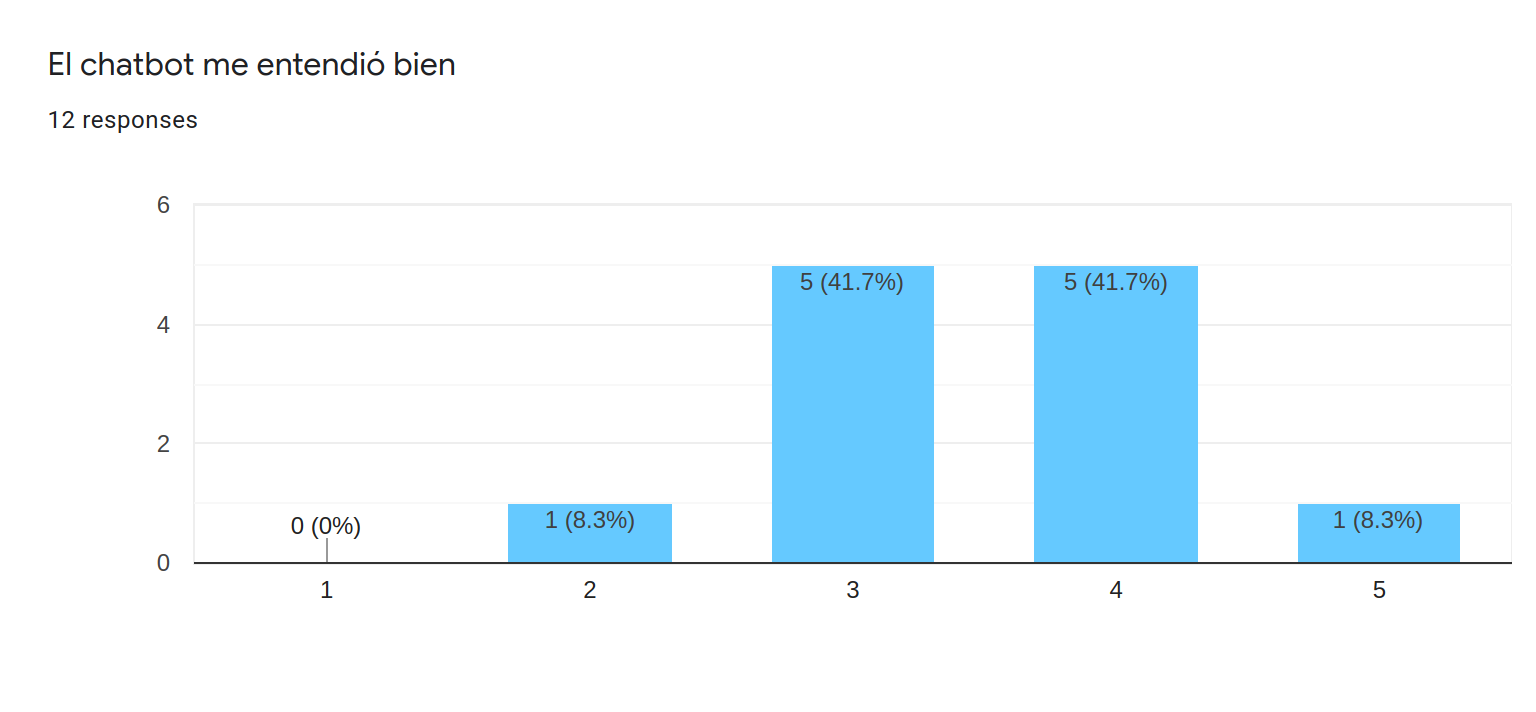
\includegraphics[scale=0.3]{../images/pregunta3.png}
\caption{Valoración de respuestas}
\label{fig:encuesta2}
\end{figure}

Un 41.7\% de los encuestados valoró con un 3 y un 8.3\% con un 4 su experiencia respecto a que el chatbot 	no fuera capaz de reconocer muchas de las entradas. Por tanto, al menos la mitad de los encuestados (41.7\% + 8.3\%) manifiestan que el asistente tiene aún mucho margen de mejora respecto al reconocimiento. De igual manera, se han obtenido los mismos resultados (pero invertidos) para \textit{El chatbot me entendió bien}. De nuevo, al menos un 50\% de los participantes expresó que el asistente no entendió bien en algún momento lo que querían expresar. Este hecho se ha podido corroborar analizando varias de las conversaciones recopiladas durante la prueba. En ellas, se puede observar como estos usuarios han realizado distintas preguntas que el chatbot, por falta de conocimiento, no ha sido capaz de responder o ha ofrecido una respuesta equivocada.\\



En general, los resultados del estudio de usabilidad han sido satisfactorios y el cuestionario CUQ ha permitido detectar aquellos aspectos de VIHrtual-App que necesitan mejorar. En especial, el reconocimiento de las entradas debe mejorarse y la base de conocimiento debe ampliarse.\\

